\documentclass[xcolor=table]{beamer}

% \rowcolors{1}{gray!30}{gray!10}

\usetheme{Boadilla}
\usecolortheme{dolphin}
\useoutertheme[subsection=false]{smoothbars}

\setbeamercolor{frametitle}{fg = black, bg = white} 
\setbeamercolor{palette primary}{use=structure,fg=white,bg=structure.fg!60!white}
\setbeamercolor{palette secondary}{use=structure,fg=white,bg=structure.fg!90!white}
\setbeamercolor{palette tertiary}{use=structure,fg=white,bg=structure.fg!120!white}
\setbeamercolor{palette quaternary}{use=structure,fg=black,bg=white} %Top bar

\setbeamertemplate{enumerate subitem}[circle]%
\renewcommand{\insertsubenumlabel}{\alph{enumii}}

\usepackage{amsmath}
\usepackage{xcolor}
\usepackage{booktabs}
\usepackage[utf8]{inputenc}
\usepackage{hyperref}
\usepackage[table]{xcolor}
\definecolor{lightgray}{gray}{0.9}

\hypersetup{
    colorlinks,
    citecolor=blue,
    linkcolor=blue
}

\footnotesize \let\small\footnotesize

\author{Jonathan P. Latner, PhD}
\title{GANs}
\date{\today}

\beamertemplatenavigationsymbolsempty 
\setbeamerfont{page number in head/foot}{size=\tiny}
\setbeamertemplate{footline}[frame number]
\setbeamertemplate{caption}[numbered]
\setbeamertemplate{section in toc}[sections numbered]

\begin{document}

\section{Introduction}\label{sec:intro}
\frame{\frametitle{ }
\titlepage
\thispagestyle{empty}
}

\frame[c]{\frametitle{The question}
\centering
When are GANs efficient/effective in creating synthetic data sets relative to Synthpop (Datasynthesizer)?
}

\frame{\frametitle{What do we know?}
}

\frame{\frametitle{What do we not know?}
}

\section{Categorical}\label{sec:categorical}

\frame{\frametitle{Data}
\begin{itemize}
    \item 2 rows/observations = [1.000, 5.000]
    \item 3 cols/variables = [10, 15, 20]
    \item 4 values per variable = [5, 10, 15, 20]
    \item Datasets = 24 ($2 \times 3 \times 4$)
    \item Synthpop, Datasynthesizer, CTGAN set to default values
    \item Note: 1 synthetic copy per dataset because focus is on duration
\end{itemize}
}


\frame{\frametitle{}
\begin{figure}
    \caption{Duration: CTGAN $=<$ Synthpop if (cols $>$ 20 $|$ vals $>$ 20)}
    \resizebox{\textwidth}{!}{\includegraphics{../categorical_dim/graphs/graph_compare_duration.pdf}}
    \label{}
\end{figure}
}

\frame{\frametitle{}
\begin{figure}
    \caption{Kolmogorov-Smirnov utility measure}
    \resizebox{\textwidth}{!}{\includegraphics{../categorical_dim/graphs/graph_compare_utility_ks.pdf}}
    \label{}
\end{figure}
}

\frame{\frametitle{}
\begin{figure}
    \caption{Example frequency for cols = 10, rows = 1.000, vals = 5}
    \resizebox{\textwidth}{!}{\includegraphics{../categorical_dim/graphs/graph_compare_frequency.pdf}}
    \label{}
\end{figure}
}


\section{Continuous}\label{sec:continuous}

\frame{\frametitle{Data}
\begin{itemize}
    \item 3 rows/observations = [50.000, 100.000, 200.000]
    \item 3 cols/variables = [10, 15, 20]
    \item Datasets = 9
    \begin{itemize}
        \item Different distributions, depending on \# variables 
    \end{itemize}
    \item Note: 1 synthetic copies per dataset
    \item Focus on tuning CTGAN
    \begin{itemize}
        \item epochs = [10, 20, 30, 40, 50, 75, 100]
        \item batch size = [500, 1.000, 5.000, 10.000]
    \end{itemize}
\end{itemize}
}

\frame{\frametitle{}
\begin{figure}
    \caption{Frequency for cols = 10, rows = 100.000}
    \resizebox{\textwidth}{!}{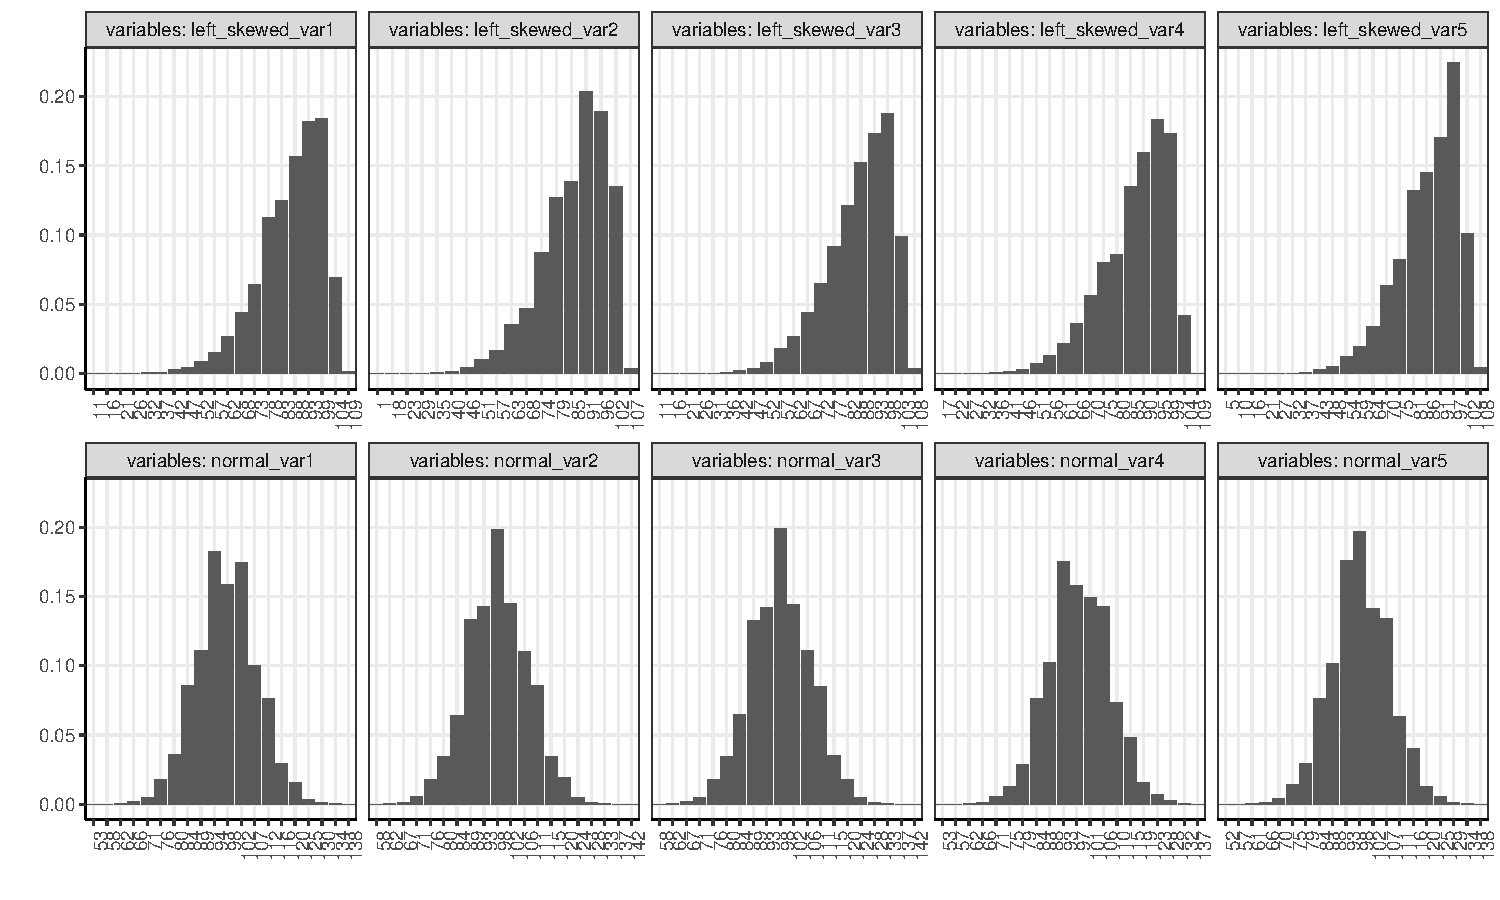
\includegraphics{../continuous_dim/graphs/graph_descriptives_rows_100000_cols_10.pdf}}
    \label{}
\end{figure}
}

\frame{\frametitle{}
\begin{figure}
    \caption{Frequency for cols = 15, rows = 100.000}
    \resizebox{\textwidth}{!}{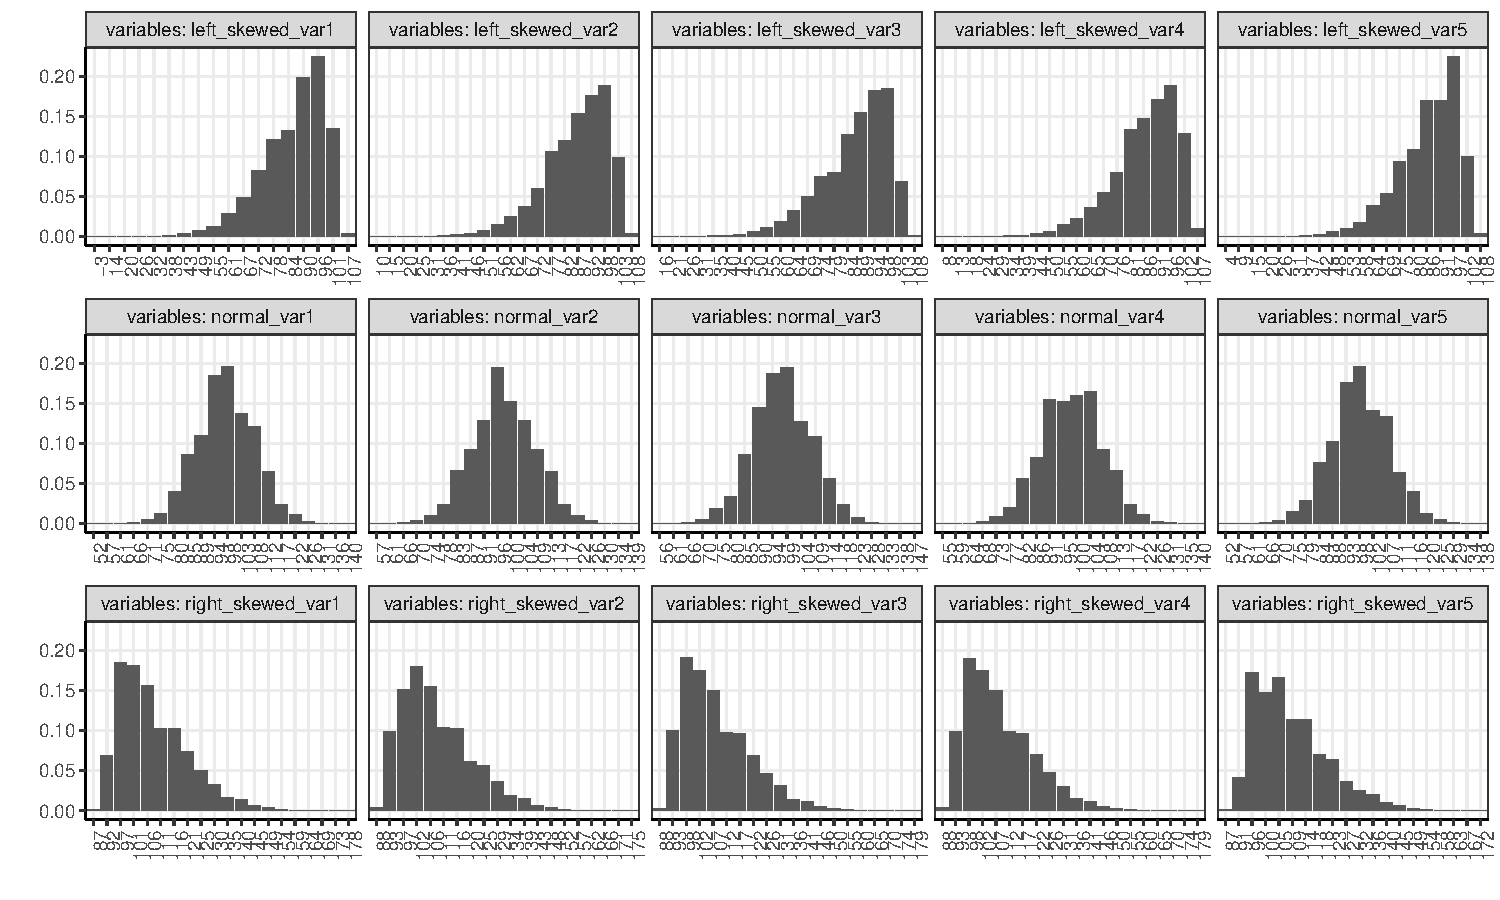
\includegraphics{../continuous_dim/graphs/graph_descriptives_rows_100000_cols_15.pdf}}
    \label{}
\end{figure}
}

\frame{\frametitle{}
\begin{figure}
    \caption{Frequency for cols = 20, rows = 100.000}
    \resizebox{\textwidth}{!}{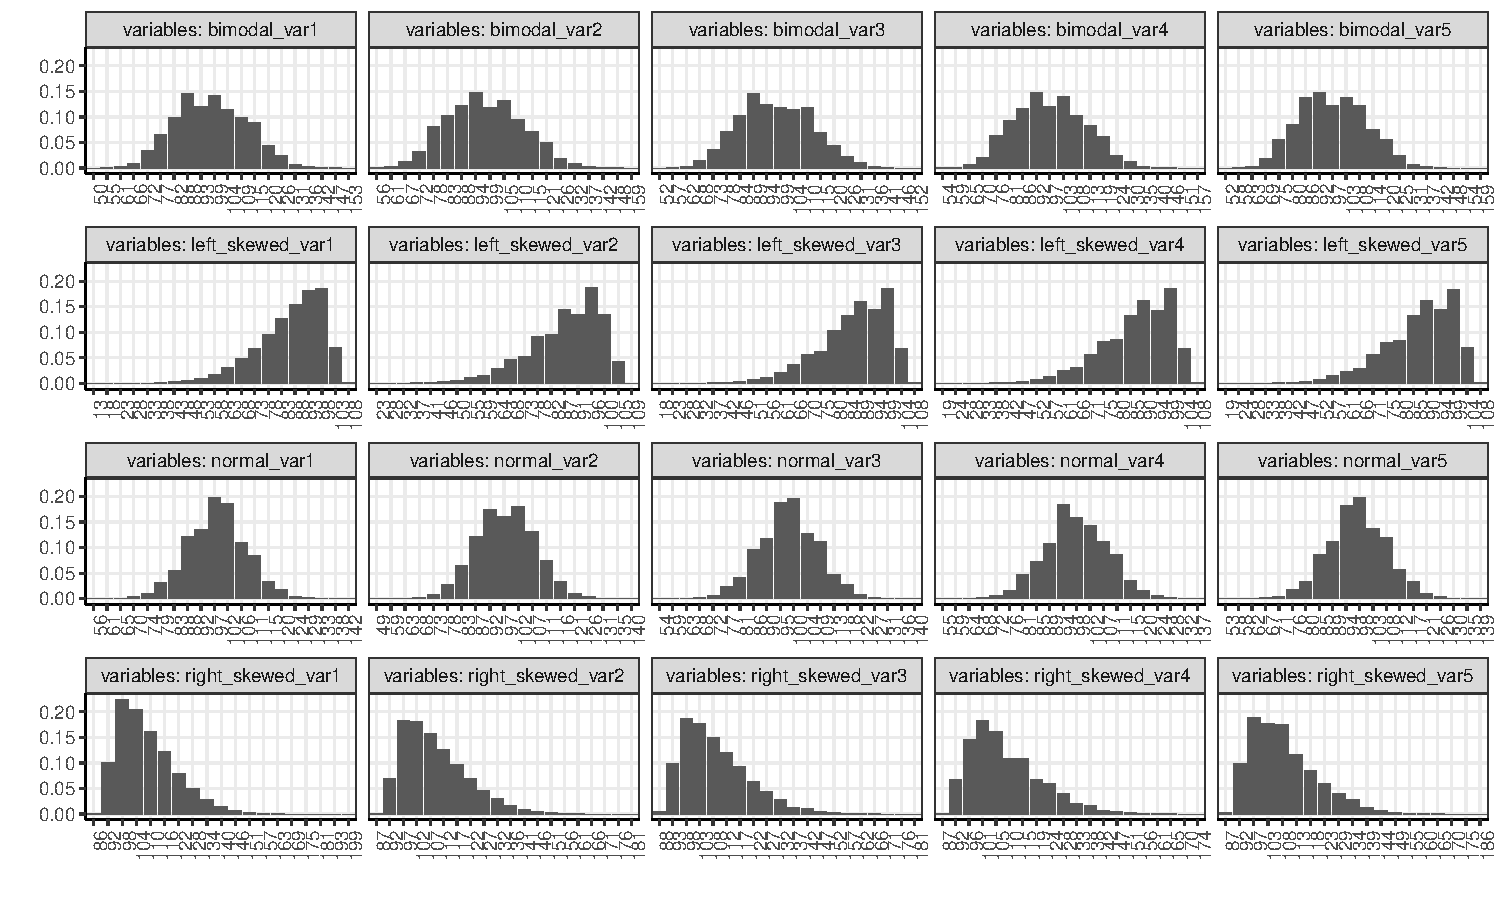
\includegraphics{../continuous_dim/graphs/graph_descriptives_rows_100000_cols_20.pdf}}
    \label{}
\end{figure}
}

\frame{\frametitle{}
\begin{figure}
    \caption{Duration (CTGAN)}
    \resizebox{\textwidth}{!}{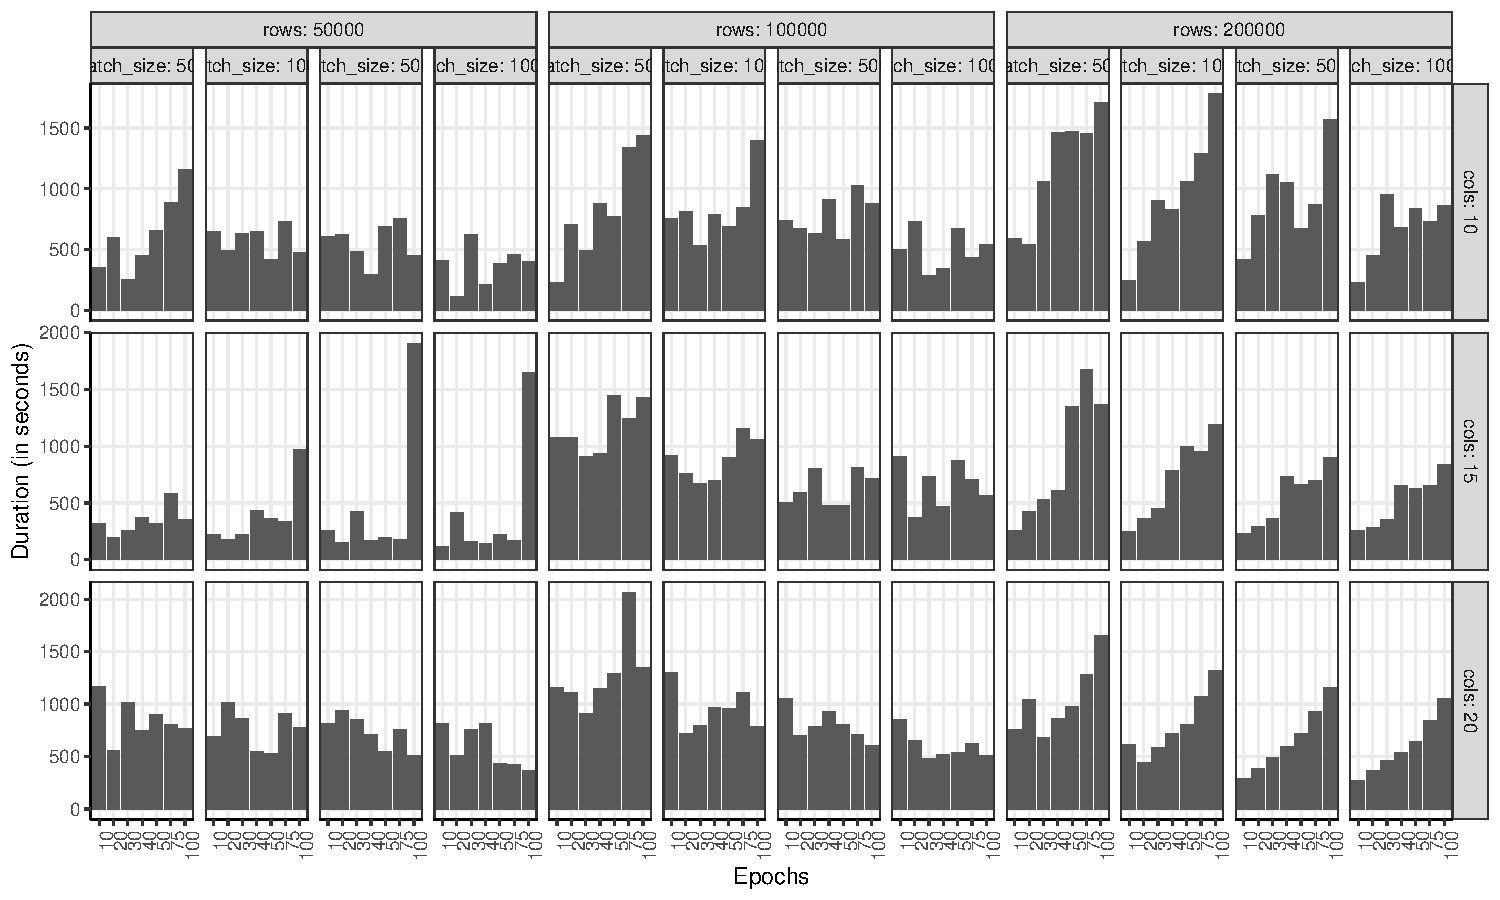
\includegraphics{../continuous_dim/graphs/graph_compare_ctgan_duration.pdf}}
    \label{}
\end{figure}
}

\frame{\frametitle{}
\begin{figure}
    \caption{Kolmogorov-Smirnov utility measure (CTGAN)}
    \resizebox{\textwidth}{!}{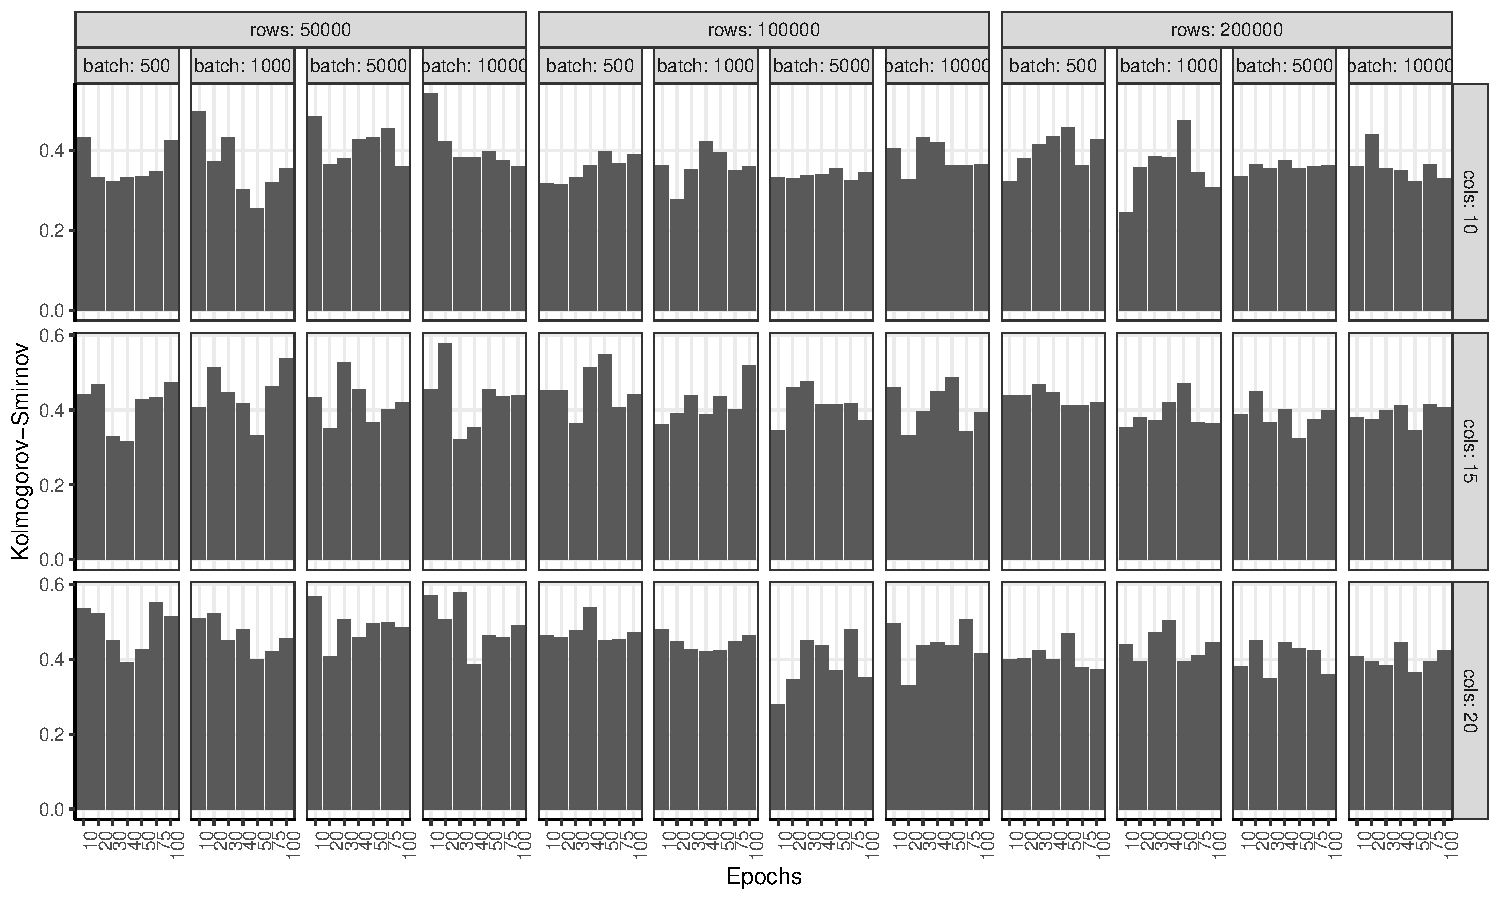
\includegraphics{../continuous_dim/graphs/graph_compare_ctgan_specks.pdf}}
    \label{graph_compare_ctgan_specks}
\end{figure}
}

\frame{\frametitle{}
\begin{figure}
    \caption{Kolmogorov-Smirnov utility measure}
    \resizebox{.9\textwidth}{!}{\includegraphics{../continuous_dim/graphs/graph_compare_utility_ks.pdf}}
    \label{}
\end{figure}
\tiny{Note: CTGAN hyperparameter: batch size = 1000 and epochs = 50 (see figure \ref{graph_compare_ctgan_specks})}
}


\frame{\frametitle{}
\begin{figure}
    \caption{Duration}
    \resizebox{.9\textwidth}{!}{\includegraphics{../continuous_dim/graphs/graph_compare_duration.pdf}}
    \label{}
\end{figure}
\tiny{Note: CTGAN hyperparameter: batch size = 1000 and epochs = 50 (see figure \ref{graph_compare_ctgan_specks})}
}

\frame{\frametitle{}
\begin{figure}
    \caption{Example frequency for cols = 10}
    \resizebox{.9\textwidth}{!}{\includegraphics{../continuous_dim/graphs/graph_compare_frequency.pdf}}
    \label{}
\end{figure}
\tiny{Note: CTGAN hyperparameter: batch size = 1000 and epochs = 50 (see figure \ref{graph_compare_ctgan_specks})}
}

% Table
% \frame{\frametitle{}
% \begin{table}[!h]
%     \caption{}
%     \centering
%     \resizebox{.9\textwidth}{!}{\input{../../tables/}}
%     \label{}
% \end{table}
% }


\end{document}


